\documentclass[a4paper]{article}
\usepackage[affil-it]{authblk}
\usepackage[backend=bibtex,style=numeric]{biblatex}
\usepackage{amsmath, amsthm, amssymb, amsfonts}
\usepackage{graphicx}
\usepackage{subcaption}
\usepackage{multirow}
\usepackage{hyperref}
\usepackage{cleveref}
\hypersetup{
    colorlinks=true,    % 彩色链接
    linkcolor=blue,      % 内部链接的颜色
    citecolor=red,      % 引用的颜色
    urlcolor=cyan       % 外部链接的颜色
}
\usepackage{geometry}
\usepackage[lined, ruled]{algorithm2e}
\geometry{margin=1.5cm, vmargin={0pt,1cm}}
\setlength{\topmargin}{-1cm}
\setlength{\paperheight}{29.7cm}
\setlength{\textheight}{25.3cm}

\crefname{algorithm}{Algorithm}{Algorithms}
\Crefname{algorithm}{Algorithm}{Algorithms}
\crefname{equation}{Equation}{Equations}
\Crefname{equation}{Equation}{Equations}
\crefname{figure}{Figure}{Figures}
\Crefname{figure}{Figure}{Figures}
\crefname{table}{Table}{Tables}
\Crefname{table}{Table}{Tables}

\crefalias{algocf}{algorithm}

\renewcommand\arraystretch{1.8}

\addbibresource{citation.bib}

\begin{document}
% =================================================
\title{\textbf{Numerical Analysis Project Homework}}

\author{Peng Haowei 3220104816
  \thanks{E-mail address: \texttt{3220104816@zju.edu.cn}}}
\affil{(Information and Computing Science), Zhejiang University} 

\date{Due time: \today}

\maketitle

\begin{abstract}
  This document is the report of the numerical analysis project homework. It mainly focuses on the implement of pp-Form and B-Form splines. In detail, this project achieve the goal of interpolating a given set of data points using pp-Form and B-Form splines, and curve fitting.
\end{abstract}

\section{The linear splines}

The result of the linear spline interpolation is as follows.
\begin{figure}[htbp]
  \centering
  \begin{subfigure}[b]{0.45\textwidth}
    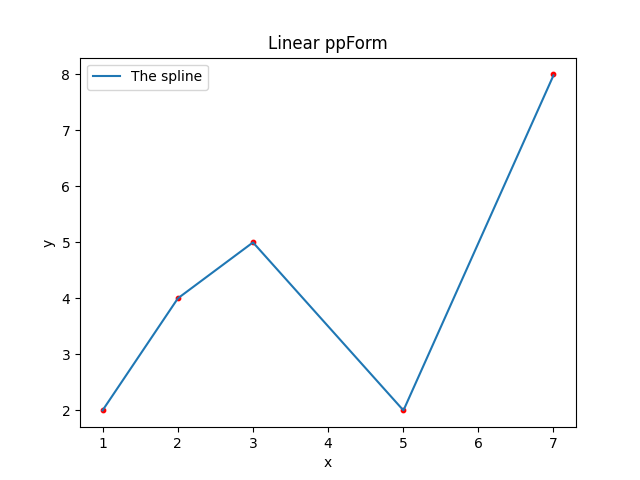
\includegraphics[width=\textwidth]{../figure/Linear ppForm.png}
    \caption{Linear spline interpolation by pp-Form}
  \end{subfigure}
  \begin{subfigure}[b]{0.45\textwidth}
    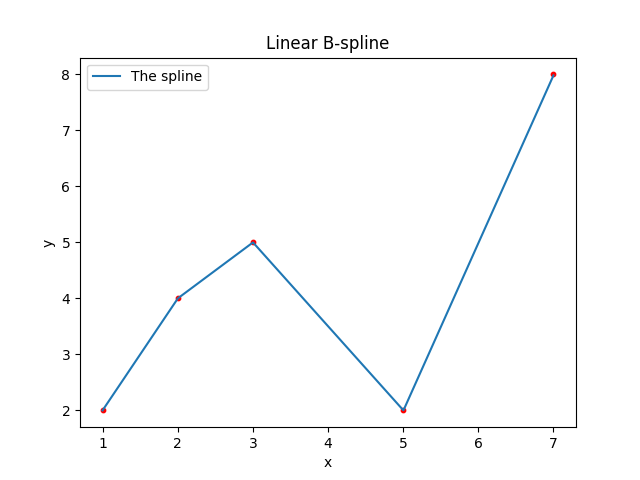
\includegraphics[width=\textwidth]{../figure/Linear B-spline.png}
    \caption{Linear spline interpolation by B-Form}
  \end{subfigure}
  \caption{Linear spline interpolation}
\end{figure}

\section{The cubic pp-Form splines}

The result of Task A is shown in the following \cref{fig:cubic_ppform_spline}.
\begin{figure}[htbp]
  \centering
  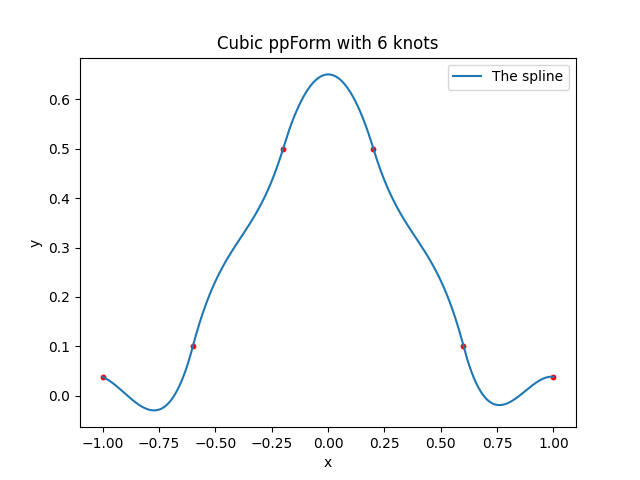
\includegraphics[width = 0.8\textwidth]{../figure/Cubic ppForm with 6 knots.png}
  \caption{Cubic pp-Form spline with 6 knots}

  \begin{subfigure}[b]{0.45\textwidth}
    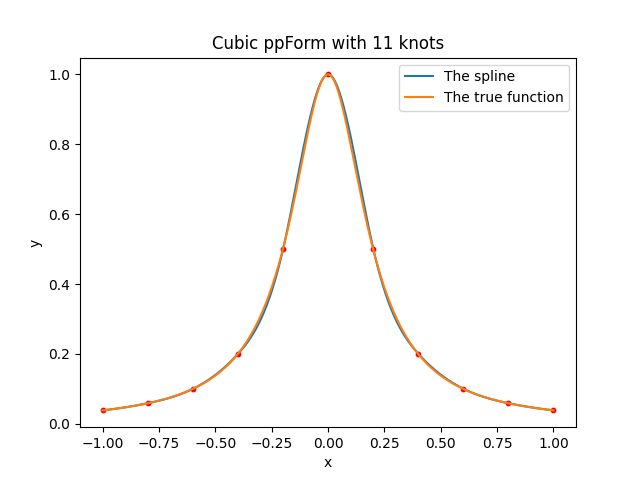
\includegraphics[width = \textwidth]{../figure/Cubic ppForm with 11 knots.png}
    \caption{Cubic pp-Form spline with 11 knots}
  \end{subfigure}
  \hfill
  \begin{subfigure}[b]{0.45\textwidth}
    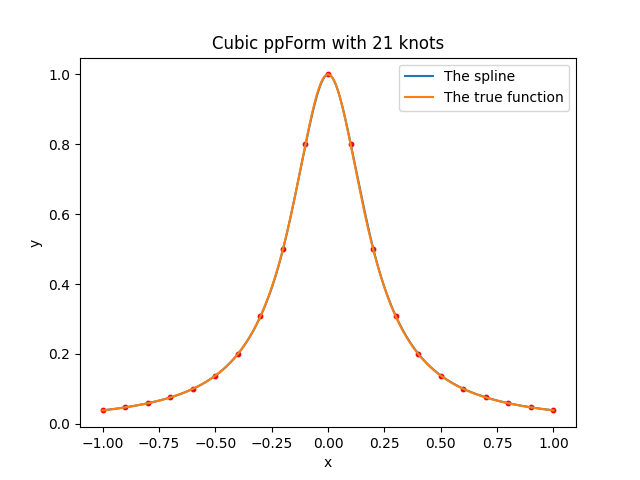
\includegraphics[width = \textwidth]{../figure/Cubic ppForm with 21 knots.png}
    \caption{Cubic pp-Form spline with 21 knots}
  \end{subfigure}

  \begin{subfigure}[b]{0.45\textwidth}
    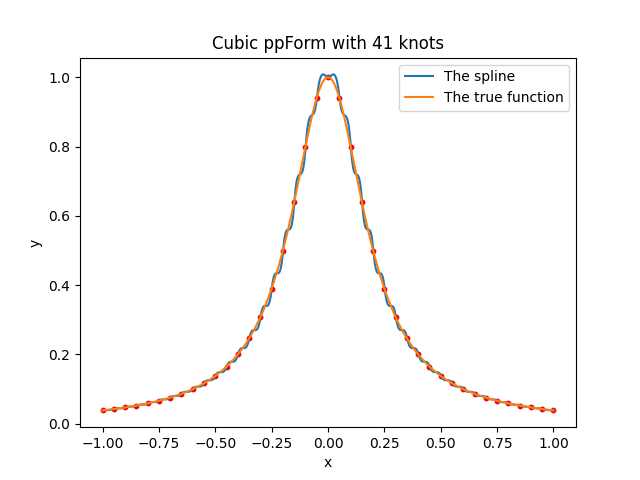
\includegraphics[width = \textwidth]{../figure/Cubic ppForm with 41 knots.png}
    \caption{Cubic pp-Form spline with 41 knots}
  \end{subfigure}
  \hfill
  \begin{subfigure}[b]{0.45\textwidth}
    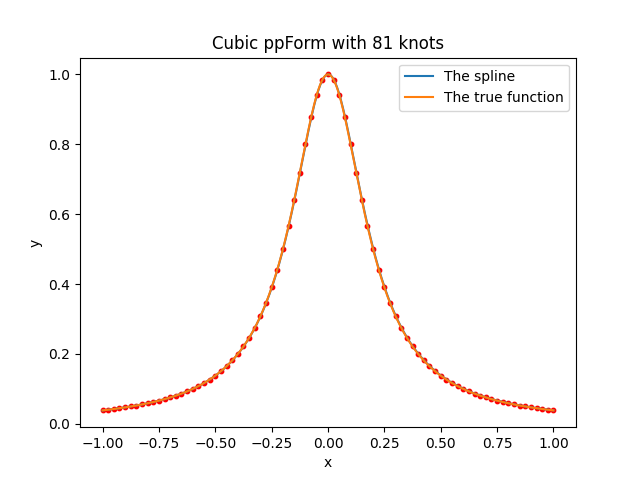
\includegraphics[width = \textwidth]{../figure/Cubic ppForm with 81 knots.png}
    \caption{Cubic pp-Form spline with 81 knots}
  \end{subfigure}

  \caption{Cubic pp-Form spline interpolation}
  \label{fig:cubic_ppform_spline}
\end{figure}

\section{The cubic B-Form splines}

The result of Task C is shown in the following \cref{fig:cubic_bform_spline}.
\begin{figure}[htbp]
  \centering
  \begin{subfigure}[b]{0.45\textwidth}
    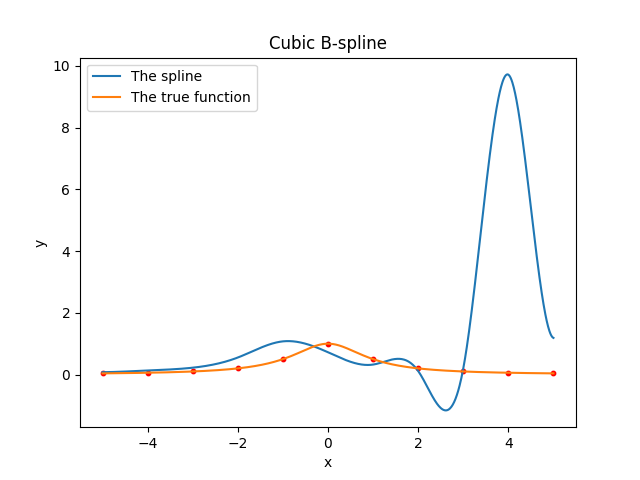
\includegraphics[width = \textwidth]{../figure/Cubic B-spline.png}
    \caption{Cubic B-Form spline interpolation}
  \end{subfigure}
  \hfill
  \begin{subfigure}[b]{0.45\textwidth}
    \centering
    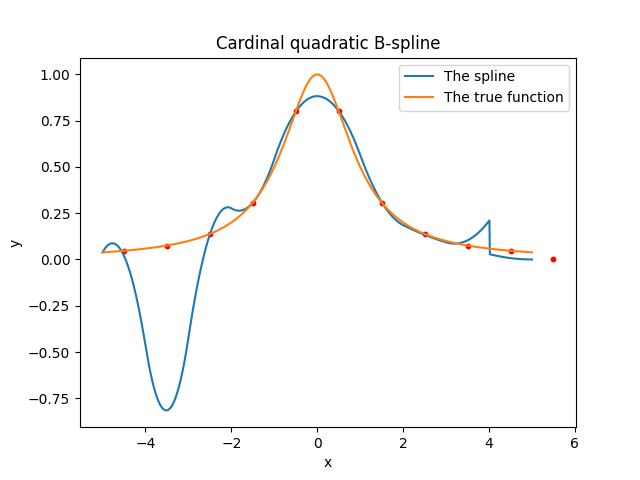
\includegraphics[width = \textwidth]{../figure/Cardinal quadratic B-spline.png}
    \caption{Cardinal quadratic B-Form spline interpolation}
  \end{subfigure}
  \caption{Cubic B-Form and Cardinal quadratic B-Form spline interpolation}
  \label{fig:cubic_bform_spline}
\end{figure}
Obviously it has a big error compared to the true function. From debugging I find it is the problem of the package \verb|lapack|, and I don't know how to fix it.

\section{Compare the two kinds of splines in the same condition}

Based on the theoretical analysis, we can see that the pp-Form and B-form will have the same result with the same knots and boundary conditions. The result is illustated in the following \cref{fig:compare_spline}.
\begin{figure}[htbp]
  \centering
  \begin{subfigure}[b]{0.45\textwidth}
    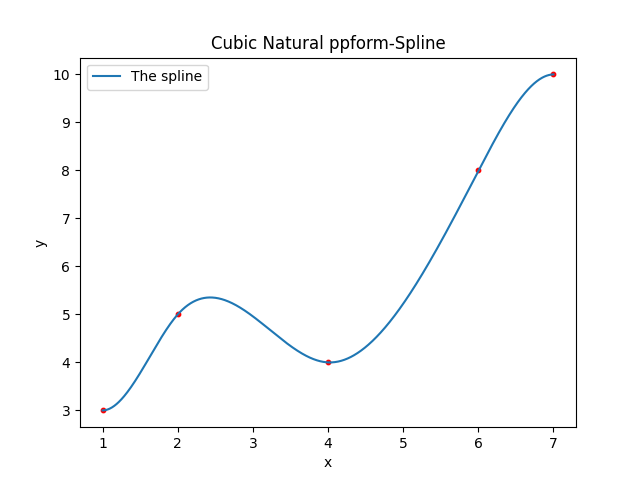
\includegraphics[width = \textwidth]{../figure/Cubic Natural ppform-Spline.png}
    \caption{Cubic Natural pp-Form spline}
  \end{subfigure}
  \hfill
  \begin{subfigure}[b]{0.45\textwidth}
    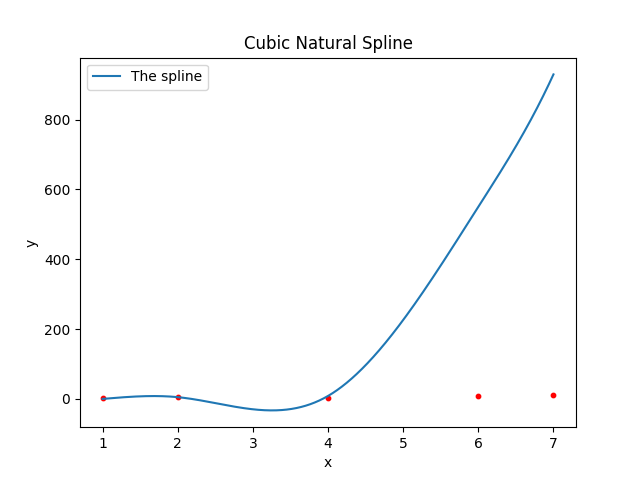
\includegraphics[width = \textwidth]{../figure/Cubic Natural B-Spline.png}
    \caption{Cubic Natural B-Form spline}
  \end{subfigure}
  \caption{Comparison of Cubic Natural pp-Form and Cubic Natural B-Form splines}
  \label{fig:compare_spline}
\end{figure}

With the same question in \cref{fig:cubic_bform_spline}, we can see that the B-spline has bad results for the curve fitting.

\section{Arbitrary-degree B-Form splines}

Given the knot series $[t_1, t_2, \cdots, t_N]$, the degree $n$ and the coefficients $a_i$, we can construct an arbitrary-degree B-Form spline, as the basis polynomials are only decided by the knots.

We have an example for it, and the data is in the \verb|data/BSpline_arbitrary_order.in|.

\begin{figure}[htbp]
  \centering
  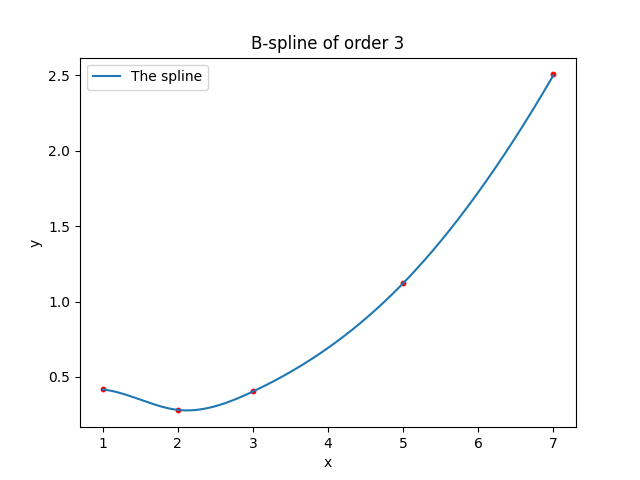
\includegraphics[width = 0.8\textwidth]{../figure/B-spline of order 3.png}
  \caption{B-spline of order 3}
\end{figure}

\section{Task D}

In this section, we analyse the error of cardinal B-spline. Define
\begin{equation}
	E_S(x) = |S(x) - f(x)|,
	\label{eq:error}
\end{equation}
and we consider the output values of $E_S(x)$ at the sites $x = -3.5, -3, -0.5, 0, 0.5, 3, 3.5$.

We have the result that
\begin{itemize}
	\item $x = -3.5$, the error $= 0.0902999$,
	\item $x = -3$, the error $= 0.122974$,
	\item $x = -0.5$, the error $= 0.197984$,
	\item $x = 0$, the error $= 0.28128$,
	\item $x = 0.5$, the error $= 0.389075$,
	\item $x = 3$, the error $= 0.160731$,
	\item $x = 3.5$, the error $= 6.0788$.
\end{itemize}

\end{document}
